
\subsection{Engelbertus Adiputra Mau Leto}
\section{Sejara Python}
              Python dikembangkan oleh Guido van Rossum pada tahun 1990 di CWI, Amsterdam sebagai kelanjutan dari bahasa pemrograman ABC. Tahun 1995, Guido pindah ke CNRI sambil terus melanjutkan pengembangan Python. Versi terakhir yang dikeluarkan adalah 1.6. Tahun 2000, Guido dan para pengembang inti Python pindah ke BeOpen.com yang merupakan sebuah perusahaan komersial dan membentuk BeOpen PythonLabs. Python 2.0 dikeluarkan oleh BeOpen. Setelah mengeluarkan Python 2.0, Guido dan beberapa anggota tim PythonLabs pindah ke DigitalCreations. Saat ini pengembangan Python terus dilakukan oleh sekumpulan pemrogram yang dikoordinir Guido dan Python Software Foundation. Python Software Foundation adalah sebuah organisasi non-profit yang dibentuk sebagai pemegang hak cipta intelektual Python sejak versi 2.1 dan dengan demikian mencegah Python dimiliki oleh perusahaan komersial. Saat ini distribusi Python sudah mencapai versi 2.6.1 dan versi 3.0. Nama Python dipilih oleh Guido sebagai nama bahasa ciptaannya karena kecintaan guido pada acara televisi Monty Python's Flying Circus. Oleh karena itu seringkali ungkapan-ungkapan khas dari acara tersebut seringkali muncul dalam korespondensi antar pengguna Python. 

\
\section{Instalasi Anaconda}
\begin{enumerate}
    \item Pastikan Bahwa Python telah terinstal dilaptop anda.
    \item Jika anda belum punya anaconda, kalian bisa download
    \item Kemudian buka installer yang telah di download barusan
    \item Klik next
    \begin{figure}[H]
        \centering
        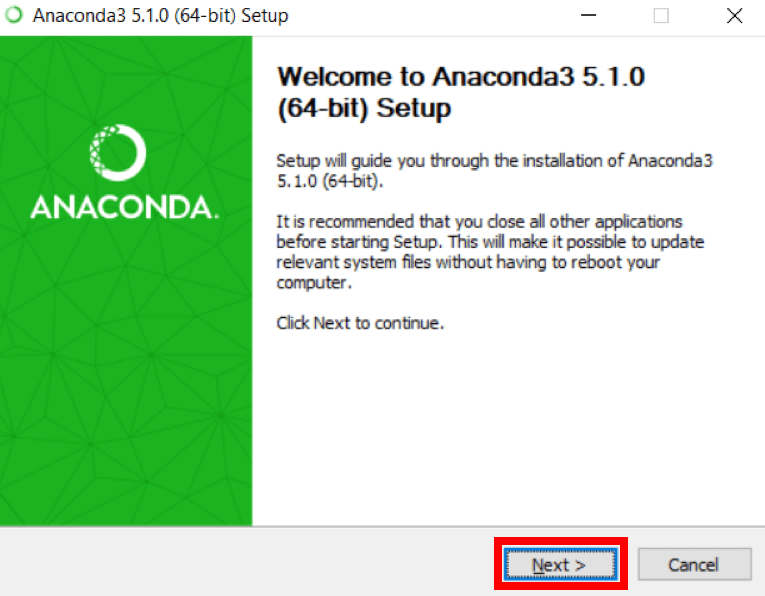
\includegraphics[width=3cm,height=3cm]{figures/1.png}
        \label{awal}
        \end{figure}

    \item klik next
    \begin{figure}[H]
        \centering
        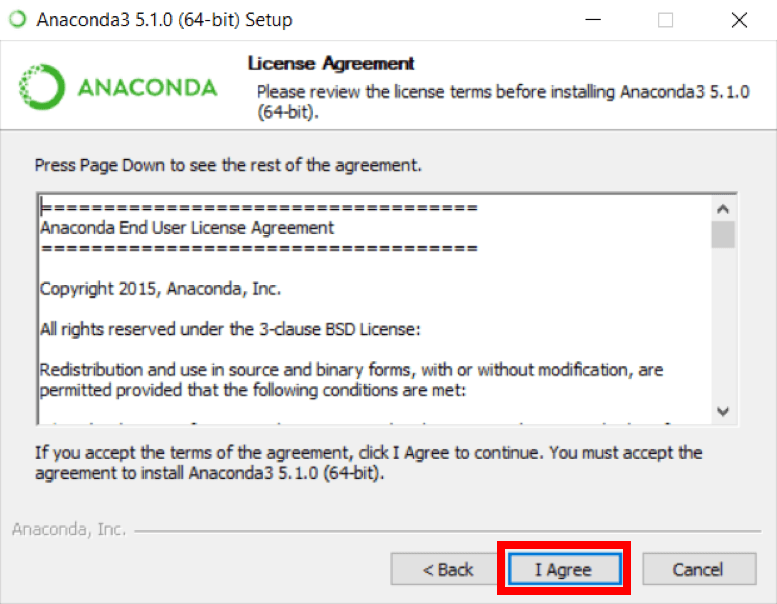
\includegraphics[width=3cm,height=3cm]{figures/2.png}
        \caption{Klik Next}
        \label{License}
        \end{figure}

    \item Klik pada I Agree
     \begin{figure}[H]
        \centering
        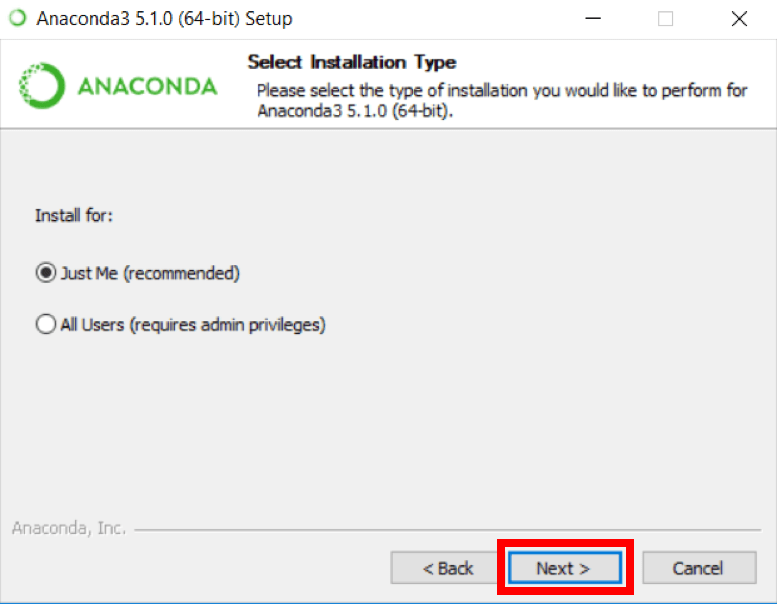
\includegraphics[width=3cm,height=3cm]{figures/3.png}
        \caption{Klik pada I Agreer}
        \label{User}
        \end{figure}

    \begin{figure}[!htbp]
        \centering
        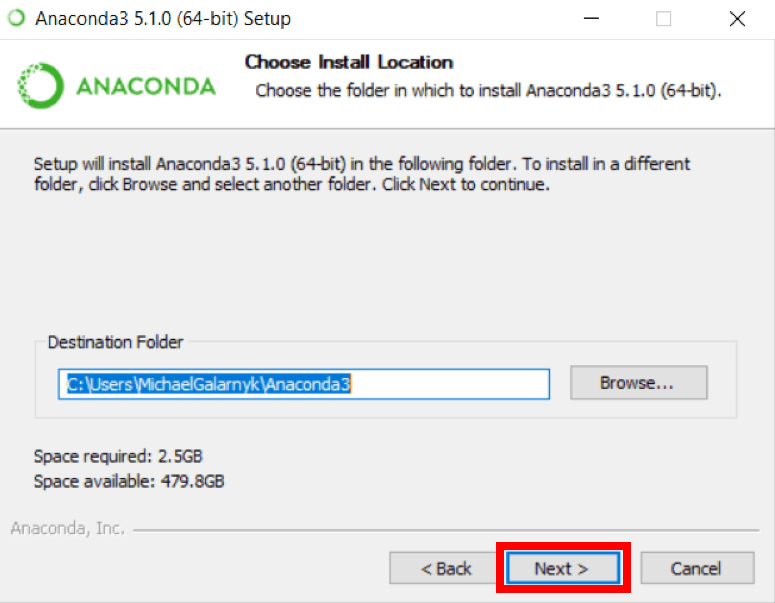
\includegraphics[width=3cm,height=3cm]{figures/4.png}
        \label{Directory}
        \end{figure}

     \begin{figure}[H]
        \centering
        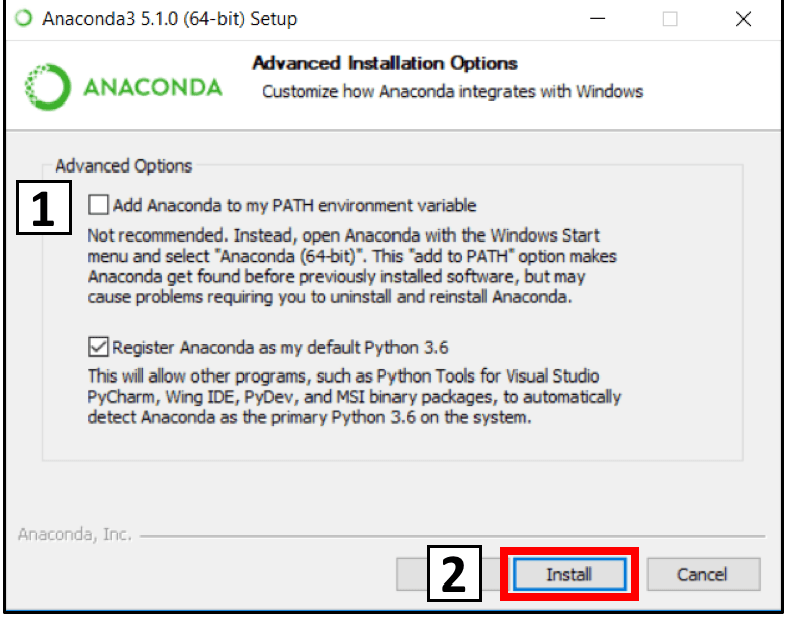
\includegraphics[width=3cm,height=3cm]{figures/5.png}
        \label{opsi}
        \end{figure}

    \item Ceklis pada Add Anaconda to my PATH environment varable dan Register Anaconda as my default Python 3.7 .selanjutnya klik Install
    \begin{figure}[H]
        \centering
        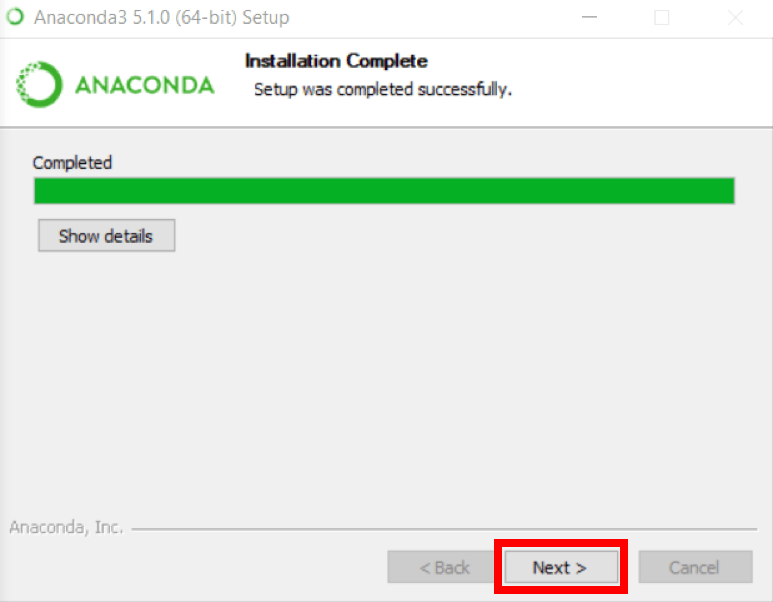
\includegraphics[width=3cm,height=3cm]{figures/6.png}
        \caption{Ceklis pada Add Anaconda to my PATH environment varable dan Register Anaconda as my default Python 3.7 .selanjutnya klik Install}
        \label{Proses}
        \end{figure}

    \item Klik next
    \begin{figure}[H]
        \centering
        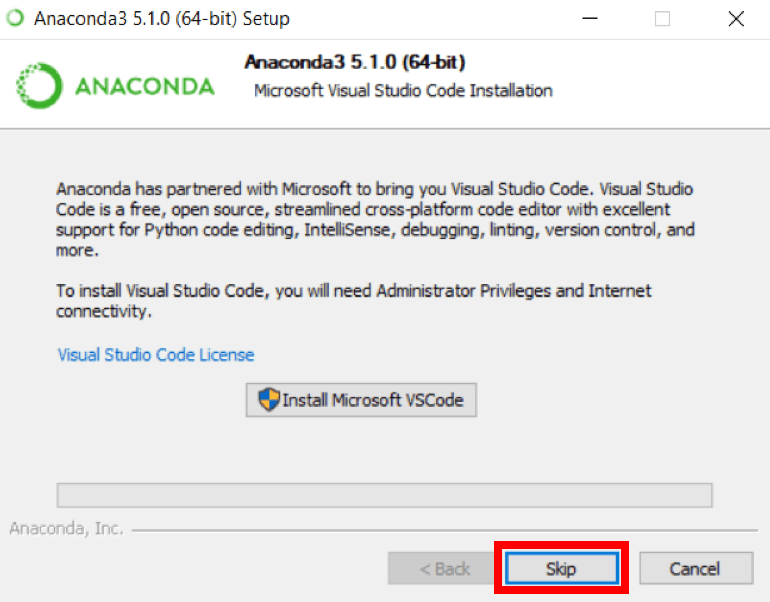
\includegraphics[width=3cm,height=3cm]{figures/7.png}
        \caption{Proses Instali}
        \label{Proses}
        \end{figure}

    \item klik next
    \begin{figure}[H]
        \centering
        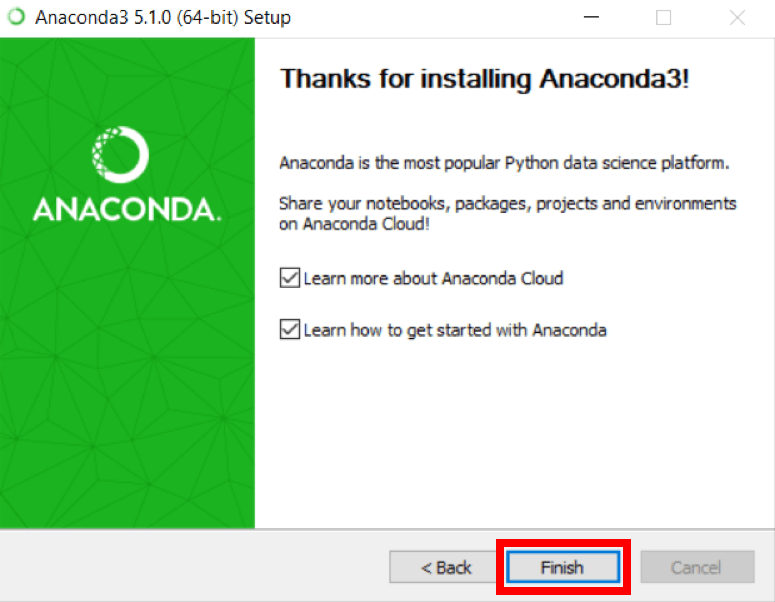
\includegraphics[width=3cm,height=3cm]{figures/8.png}
        \caption{klik next}
        \label{offering}
        \end{figure}

 \item instal MS VSC di sarankan menginstalnya dulu
    \begin{figure}[H]
        \centering
        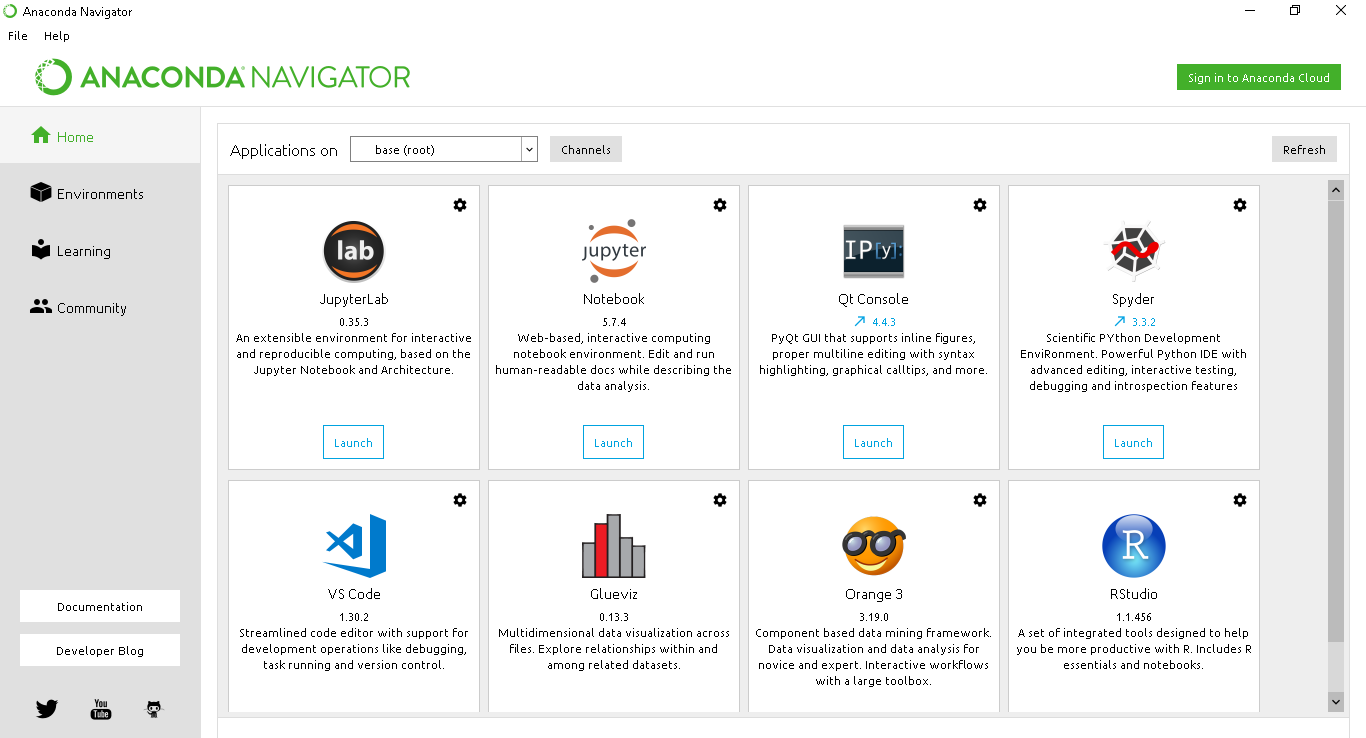
\includegraphics[width=3cm,height=3cm]{figures/9.png}
        \caption{Klik install microsoft vscode}
        \label{offering}
        \end{figure}

    \item Instalasi anaconda telah selesai
     \begin{figure}[H]
        \centering
        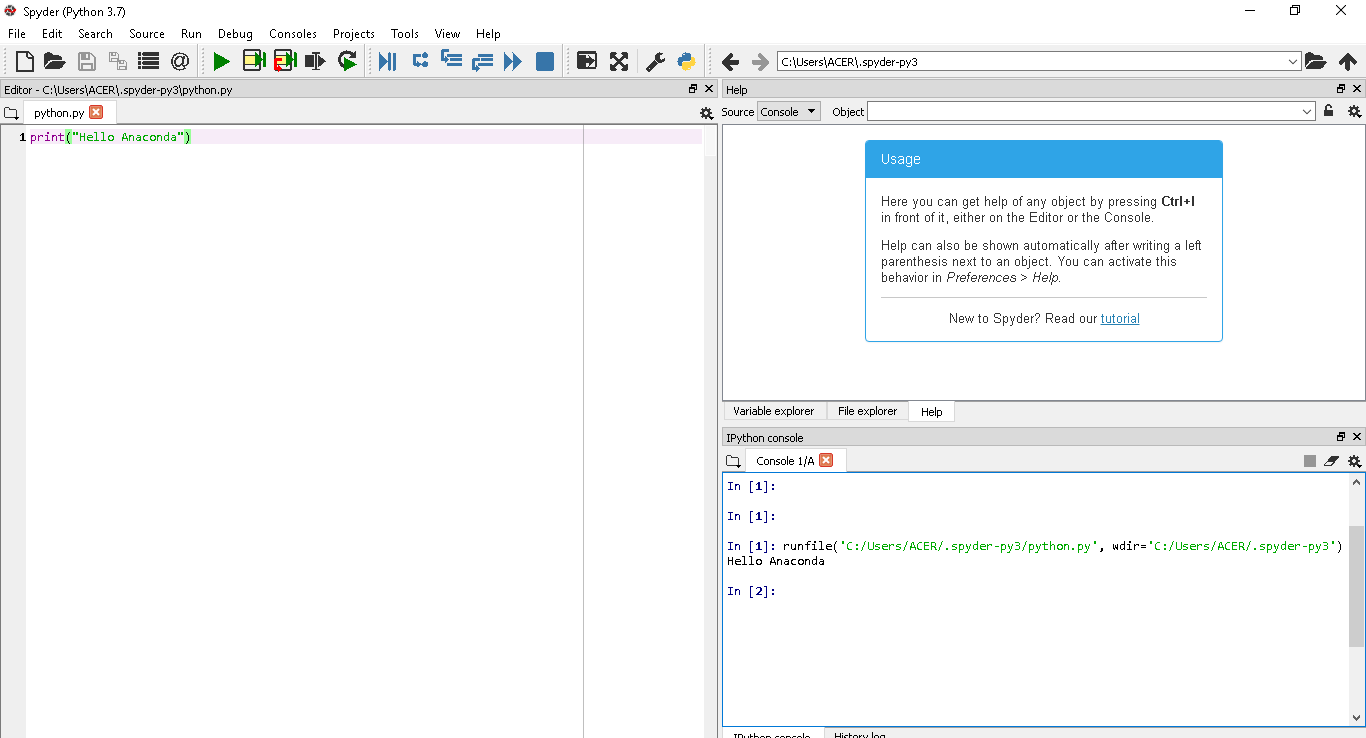
\includegraphics[width=3cm,height=3cm]{figures/10.png}
        \caption{Instalasi Selesai}
        \label{akhir}
        \end{figure}
\end{enumerate}

\section{Menggunakan Spyder}

     \begin{figure}[H]
        \centering
        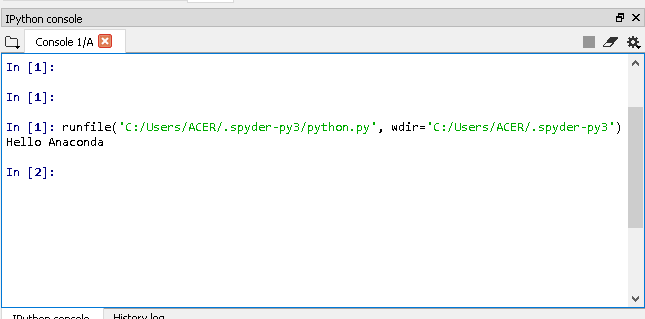
\includegraphics[width=3cm,height=3cm]{figures/11.PNG}
        \label{akhir}
        \end{figure}

\end{document}